\scanpage{37}
\margin{36}
the square is
\[
 \lambda=\frac{(\xi+\eta)^2}{\xi\wedge\eta}
 =\deleted{\unsure{\frac{\xi}{\eta}}}\frac{\xi}{\eta}+\frac{\eta}{\xi}+2
\]
and knowledge of which allows us to recover the initial situation up to
\uline{\unsure{a|to the}} \uline{unique} isomorphism. The condition to impose on
$\lambda$ is that $\lambda-4\ne0$ i.e.
\[
 \lambda'\overset{\unsure{\mathrm{df}}}{=}\lambda-
 2= \frac{\xi}{\eta}+\frac{\eta}{\xi}\ne2
\]
In terms of a basis \deleted{\unsure{of}} $e_1$ of $L_1$,
satisfying $e_1^4=e=\xi\wedge\eta$, giving a basis $e_1^2$ of $L_2$,
the situation is determined by \inserted{the pair of distinct elements}
$\xi_0,\eta_0\in\mathbb C$ $(\xi=\xi_0e_1^2,\ \eta=\eta_0e_1^2)$,
satisfying $\xi_0\eta_0=1$, or again by
$\mu=\xi_0+\eta_0\inserted{\in\mathbb C}$, satisfying $\mu^2-4\ne0$,
$\xi_0$ and $\eta_0$ being recovered as solutions of the equation
\[
 z^2-\mu z+1=0,
\]
the equation \tikz[baseline=(ineq.base)]{
\node[inner sep=1pt] (ineq) {$\mu^2-4\ne0\quad\text{i.e.}\quad\unsure{\mu^2|\mu}\ne\pm2$};
\draw ([xshift=-2pt,yshift=4pt]ineq.south west)
 .. controls ([xshift=-2pt,yshift=-2pt]ineq.south west) and
 ([xshift=-1pt,yshift=-3pt]ineq.south west) .. ([xshift=2pt,yshift=-3pt]ineq.south west)
 -- ([xshift=-2pt,yshift=-3pt]ineq.south east)
 .. controls ([xshift=1pt,yshift=-3pt]ineq.south east) and
 ([xshift=2pt,yshift=-1pt]ineq.south east) .. ([xshift=2pt,yshift=1pt]ineq.south east);
\draw ([xshift=5pt,yshift=2pt]ineq.south east) -- ([xshift=5pt,yshift=2pt]ineq.north east);
}
is expressed by the \inserted{2} solutions are distinct (necessaril\textsuperscript{y} nonzero since their
product is $1$). \deleted{\unsure{The}} We recover $I$ as the set of solutions of
\[
 z^4-\mu z^2+1=0
\]
\[
 I=\left\{\pm\sqrt{\tfrac12\left(\mu\pm\sqrt{\mu^2-4}\right.}\right\}
 =\left\{\pm\sqrt{\mu'\pm\sqrt{\mu'^2-1}}\right\}
\]
\margin{\begin{tikzpicture}[baseline=(eq.base)]
\node[inner sep=1pt] (eq) {where $\mu'=\tfrac12\mu$};
\node[anchor=west,inner sep=1pt] (ie) at (eq.east) {i.e.};
\draw ([xshift=-2pt]eq.west)
 .. controls ([xshift=2pt,yshift=3pt]eq.north west) and
 ([xshift=-4pt,yshift=4pt]eq.north east) .. ([xshift=0pt,yshift=2pt]eq.north east)
 .. controls ([xshift=2pt]eq.north east) and
 ([xshift=-2pt,yshift=-2pt]ie.south west) .. ([xshift=2pt,yshift=-2pt]ie.south west)
 -- ([yshift=-2pt]ie.south east);
\end{tikzpicture}}
